\documentclass{article}

% if you need to pass options to natbib, use, e.g.:
%     \PassOptionsToPackage{numbers, compress}{natbib}
% before loading neurips_2026

% The authors should use one of these tracks.
% Before accepting by the NeurIPS conference, select one of the options below.
% 0. "default" for submission
%\usepackage{neurips_2026}
\usepackage[preprint]{neurips_2026}
% the "default" option is equal to the "main" option, which is used for the Main Track with double-blind reviewing.
% 1. "main" option is used for the Main Track
%  \usepackage[main]{neurips_2026}
% 2. "position" option is used for the Position Paper Track
%  \usepackage[position]{neurips_2026}
% 3. "eandd" option is used for the Evaluations & Datasets Track
 % \usepackage[eandd]{neurips_2026}
% 4. "creativeai" option is used for the Creative AI Track
%  \usepackage[creativeai]{neurips_2026}
% 5. "sglblindworkshop" option is used for the Workshop with single-blind reviewing
 % \usepackage[sglblindworkshop]{neurips_2026}
% 6. "dblblindworkshop" option is used for the Workshop with double-blind reviewing
%  \usepackage[dblblindworkshop]{neurips_2026}
% 7. "education" option is used for the Education Track
%  \usepackage[education]{neurips_2026}


% After being accepted, the authors should add "final" behind the track to compile a camera-ready version.
% 1. Main Track
 % \usepackage[main, final]{neurips_2026}
% 2. Position Paper Track
%  \usepackage[position, final]{neurips_2026}
% 3. Evaluations & Datasets Track
 % \usepackage[eandd, final]{neurips_2026}
% 4. Creative AI Track
%  \usepackage[creativeai, final]{neurips_2026}
% 5. Workshop with single-blind reviewing
%  \usepackage[sglblindworkshop, final]{neurips_2026}
% 6. Workshop with double-blind reviewing
%  \usepackage[dblblindworkshop, final]{neurips_2026}
% Note. For the workshop paper template, both \title{} and \workshoptitle{} are required, with the former indicating the paper title shown in the title and the latter indicating the workshop title displayed in the footnote.
% For workshops (5., 6.), the authors should add the name of the workshop, "\workshoptitle" command is used to set the workshop title.
% \workshoptitle{WORKSHOP TITLE}
% 7. Education Track
% \usepackage[education, final]{neurips_2026}

% "preprint" option is used for arXiv or other preprint submissions
 % \usepackage[preprint]{neurips_2026}

% to avoid loading the natbib package, add option nonatbib:
%    \usepackage[nonatbib]{neurips_2026}

\usepackage[utf8]{inputenc} % allow utf-8 input
\usepackage[T1]{fontenc}    % use 8-bit T1 fonts
\usepackage{hyperref}       % hyperlinks
\usepackage{url}            % simple URL typesetting
\usepackage{booktabs}       % professional-quality tables
\usepackage{amsfonts}       % blackboard math symbols
\usepackage{nicefrac}       % compact symbols for 1/2, etc.
\usepackage{microtype}      % microtypography
\usepackage{xcolor}         % colors
\usepackage{graphicx}
\usepackage{amsmath}


% Note. For the workshop paper template, both \title{} and \workshoptitle{} are required, with the former indicating the paper title shown in the title and the latter indicating the workshop title displayed in the footnote. 
\title{Advanced Topics in Machine Learning PA1}


% The \author macro works with any number of authors. There are two commands
% used to separate the names and addresses of multiple authors: \And and \AND.
%
% Using \And between authors leaves it to LaTeX to determine where to break the
% lines. Using \AND forces a line break at that point. So, if LaTeX puts 3 of 4
% authors names on the first line, and the last on the second line, try using
% \AND instead of \And before the third author name.


\author{%
  Zainab Amir \\
  Department of Computer Science\\
  Lahore University of Management Sciences\\
  \texttt{28100166@lums.edu.pk} \\
  % examples of more authors
  % \And
  % Coauthor \\
  % Affiliation \\
  % Address \\
  % \texttt{email} \\
  % \AND
  % Coauthor \\
  % Affiliation \\
  % Address \\
  % \texttt{email} \\
  % \And
  % Coauthor \\
  % Affiliation \\
  % Address \\
  % \texttt{email} \\
  % \And
  % Coauthor \\
  % Affiliation \\
  % Address \\
  % \texttt{email} \\
}


\begin{document}


\maketitle


\begin{abstract}
This study explores four different areas, namely inductive biases, Unsupervised Domain Adaptation, Domain Generalization, and open-set recognition across one common objective. The aim is to understand and evaluate how robust representations are under changes in appearance, domain, and semantic novelty. Inductive biases were explored through controlled interventions varying colour, shape, texture, position and global structure and examining ResNet, CLIP, and ViT's reliance on said visual cues. The results showed more robustness to colour and translation changes compared to patch shuffling, which produced larger accuracy drops. After that, UDA on the PACS dataset showed slight improvement in Sketch accuracy over source-only ERM using DAN but also produced negative transfer in the case of adversarial methods. This was followed by the DG experiment, which showed the adverse effects of excessive domain alignment resulting in model collapse and loss of class-discriminative information. Lastly, the OSR experiments showed that stronger closed-set classification did not automatically guarantee better unknown rejection, with semantically near unknowns remaining more difficult than far unknowns. Overall, the results produced by this study suggest that robust representations must be invariant to minor, non-class-interfering changes, they must maintain class-discriminative structure, and also reject inputs not belonging to known classes. \url{https://github.com/Zeeba1705/atml_PA1}

\end{abstract}



% ============================================================
% INTRODUCTION
% ============================================================

\section{Introduction}
\label{sec:introduction}
In this study we aim to take a step beyond standard supervised learning and explore the behaviour of models that are exposed to training and test data from two different distributions, or different label spaces. This is explored across four tasks with four broad areas covered by each task respectively:  Inductive biases, Unsupervised Domain Adaptation (UDA), Domain Generalization (DG), and Open-set Recognition (OSR).Firstly, we will use controlled interventions to study how ResNets, Vision Transformers, and CLIP depend on certain visual cues in order to understand which models are biased towards shape, texture or colour, and then use patch shuffling to get an idea regarding the importance of global organisation versus locality. Feature representations will also be inspected, visualised, and potential changes will be compared to changes in predictions. In the longer run we intend on using these findings to understand what exactly a model should preserve for robust representations. 

Another question however arises from this initial question, exactly which information should be preserved under domain shift? This is one of the many questions we aim to answer using UDA and DG in tasks 2 and 3, by observing potential failures during domain shifts and connecting them to the feature representation level. Furthermore, the relationship between domain separability and recognition under domain shift, alongside its connection to class-discriminative information will be studied in depth, followed by a comparison of UDA and DG in terms of importance of unlabelled target-domain data.

While preservation and invariance are both very important in terms of robust representations, we must not forget the significance of a model being capable of rejecting inputs not belonging to one of its known classes. This concept is exactly what we explore in Task 4 using OSR, starting from differences in acceptance between near and far unknowns, using different post-hoc novelty scores to distinguish known from unknown, and finally understanding the trade-offs between closed-set accuracy and rejection performance.

Finally by the end of this study, we aim to answer the following research question which encapsulates the motivation behind performing all four tasks: “what should a robust representation preserve, what should it become invariant to, and when should it reject an input rather than force a prediction?”



\section{Experimental Setup and Methods}
\label{sec:methods}
The exact configurations, hyperparameters and splits for each task can be found in detail in the README file included in the GitHub Repository linked in this report.

\subsection{Task 1: Inductive Biases and Feature Representations}
\label{subsec:methods-task1}

Three pretrained backbones were used: ResNet-50, ViT-B/16, and CLIP ViT-B-32, on the STL-10 dataset. A linear classifier head was trained for each frozen backbone (ResNet-50, ViT, CLIP-Linear) for up to 50 epochs with early stopping; CLIP Zero-shot instead used the fixed prompt ``a photo of a \{class\}.'' All four were evaluated on top-1 accuracy, macro-F1, and mean maximum confidence, which served as the reference for the following interventions:

\begin{itemize}
    \item \textbf{Color Bias:} A grayscale transformation was applied, followed by LAB palette transfer with the palette extracted from one STL-10 image.
    \item \textbf{Shape vs.\ Texture:} 250 cue-conflict images were constructed using AdaIN ($\alpha = 1.0$) \citep{huang2017adain} across 5 class pairs, of which 50 were rejected under a visual rejection rule. Shape bias and coverage were recorded (\eqref{eq:shape_bias}, \eqref{eq:coverage}).
    \item \textbf{Translation:} Each image was translated by 0, 8, 16, and 32 pixels in the four cardinal directions via reflection padding and a shifted crop; results were averaged and prediction consistency recorded (\eqref{eq:consistency}).
    \item \textbf{Patch Structure:} Each image was divided into a $4 \times 4$ pixel-space grid and patch-shuffled.
\end{itemize}

Representation analysis was conducted by comparing each transformed image against its clean counterpart, followed by a UMAP visualization and cosine stability measurement. (\eqref{eq:cosine_stability}).

\subsection{Task 2: Unsupervised Domain Adaptation}
\label{subsec:methods-task2}
 
PACS was used to study unsupervised domain adaptation, with Sketch as the target domain and Photo, Art Painting, and Cartoon as the three source domains. Sketch images were available without labels during adaptation; target labels were used only for final evaluation. An ImageNet-pretrained ResNet-18 had its classifier replaced with a seven-class linear head and was fine-tuned under each of the following methods:
 
\begin{itemize}
    \item \textbf{Source-only ERM:} ResNet-18 and its classifier head were trained on the three labelled source domains.
    \item \textbf{DAN:} \citep{long2015learning}: MMD (\eqref{eq:mmd}) was applied to the 512-dimensional feature before the classifier to align source and target distributions, with $\lambda_{\text{MMD}} = 1$ for the main comparison. A controlled study varied $\lambda_{\text{MMD}} \in \{0.1, 1, 10\}$.
    \item \textbf{DANN:} \citep{ganin2016domain}: A binary source-vs-target domain discriminator was attached to the same feature via a gradient-reversal layer with schedule \eqref{eq:grl}. Gradient clipping and L2 feature normalization were used.
    \item \textbf{CDAN:} \citep{long2018conditional}: The discriminator was instead conditioned on both the feature and the classifier's probability vector via the outer product $g(x) = \text{vec}(f \otimes p)$ (\eqref{eq:cdan}), following the same discriminator and gradient-reversal schedule as DANN. Gradient clipping was used, with no feature normalisation.
\end{itemize}
 
BatchNorm running statistics were frozen at their pretrained ImageNet values for all methods, while the scale and bias parameters remained trainable. After training, domain separability was measured on frozen representations using a logistic-regression domain classifier.
 
\subsection{Task 3: Domain Generalization}
\label{subsec:methods-task3}
 
The same PACS source domains and pretrained ResNet-18 were used, but no Sketch images or labels were used during training, checkpoint selection, or hyperparameter selection. The Source-only ERM checkpoint from Task 2 was reused unchanged as the baseline for the following methods:
 
\begin{itemize}
    \item \textbf{DAN-DG:}\citep{long2015learning}: The model was trained using the same MMD mechanism used in Task 2, but this time to align pairs of source domains with each other rather than with Sketch (\eqref{eq:dandg}). A controlled study was also conducted by varying $\lambda_{\text{DG}} \in \{0.1, 1, 10\}$.
    \item \textbf{SAM:} The model was trained using Sharpness-Aware Minimization \citep{foret2021sharpness} with $\rho = 0.05$, requiring two forward/backward passes, with the same BatchNorm policy used during both passes.
\end{itemize}
 
The learned representations were then frozen, and a three-way logistic-regression classifier was used to distinguish between the three source domains, giving the source-domain separability score (chance level 33.3\%).
 
\subsection{Task 4: Open-Set Recognition}
\label{subsec:methods-task4}
 
Two datasets were used: CIFAR-10, providing the ten known classes, and fixed CIFAR-100 classes for unknown-class evaluation, split into near- and far-semantic groups. CIFAR-100 classes were not used in training, checkpoint selection, or score design at any point. A CIFAR-adapted ResNet-18 was used throughout, with the ImageNet $7 \times 7$, stride-2 first convolution replaced by a $3 \times 3$, stride-1 convolution and the initial max-pooling layer removed. The following experiments were conducted:
 
\begin{itemize}
    \item \textbf{Vanilla Closed-Set Baseline:} ResNet-18 was trained from random initialization with cross-entropy, then frozen to obtain logits and features used to compute four post-hoc novelty scores: MSP, MLS, Energy, and Mahalanobis (formulae in Appendix~\ref{app:formulae}). Mahalanobis class means and a shared diagonal covariance were estimated from unaugmented CIFAR-10 training features.
    \item \textbf{GCSC:} The same architecture and recipe were used, with RandAugment (\texttt{num\_ops=2}, \texttt{magnitude=9}) added to the training augmentation pipeline, evaluated using MLS.
    \item \textbf{PROSER:} \citep{zhou2021proser}: The model was initialized from the selected Vanilla checkpoint, and five dummy classifiers were added. Two placeholder objectives were used: classifier placeholders ($\beta = 1$), and data placeholders ($\gamma = 0.1$) constructed via manifold mixup \citep{verma2019manifold} between representations of different classes after \texttt{layer2}. PROSER was evaluated twice: once using MLS on the ten known-class logits, and once using its placeholder-based detection score.
\end{itemize}
 
Rejection thresholds were calibrated per model and score as the 95th percentile of unknownness on the CIFAR-10 validation set, targeting 95\% known acceptance. Closed-set accuracy, known acceptance, near/far rejection rates, and AUROC were recorded for all experiments.

% \subsection{Task 2: Unsupervised Domain Adaptation}
% PACS was used to study unsupervised domain adaptation, with Sketch as the target domain and Photo, Art Painting, and Cartoon as the three source domains. Sketch images were available without labels during adaptation; target labels were used only for final evaluation. An ImageNet-pretrained ResNet-18 had its classifier replaced with a seven-class linear head and was fine-tuned under each of the following methods:

% \textbf{Source-only ERM.} ResNet-18 and its classifier head were trained on the three labelled source domains.

% \textbf{DAN.} MMD (\eqref{eq:mmd}) was applied to the 512-dimensional feature before the classifier to align source and target distributions, with $\lambda_{\text{MMD}} = 1$ for the main comparison. A controlled study varied $\lambda_{\text{MMD}} \in \{0.1, 1, 10\}$.

% \textbf{DANN.} A binary source-vs-target domain discriminator was attached to the same feature via a gradient-reversal layer with schedule \eqref{eq:grl}. Gradient clipping and L2 feature normalisation were used.

% \textbf{CDAN.} The discriminator was instead conditioned on both the feature and the classifier's probability vector via the outer product $g(x) = \text{vec}(f \otimes p)$ (\eqref{eq:cdan}), following the same discriminator and gradient-reversal schedule as DANN. Gradient clipping was used, with no feature normalisation.

% BatchNorm running statistics were frozen at their pretrained ImageNet values for all methods, while the scale and bias parameters remained trainable. After training, domain separability was measured on frozen representations using a logistic-regression domain classifier.

% \subsection{Task 3: Domain Generalization}
% \label{subsec:methods-task3}
% The same PACS source domains and pretrained ResNet-18 were used, but no Sketch images or labels were used during training, checkpoint selection, or hyperparameter selection. The Source-only ERM checkpoint from Task 2 was reused unchanged as the baseline for the following methods:

% \textbf{DAN-DG.} The model was trained using the same MMD mechanism used in Task 2, but this time to align pairs of source domains with each other rather than with Sketch (\eqref{eq:dandg}). A controlled study was also conducted by varying $\lambda_{\text{DG}} \in \{0.1, 1, 10\}$.

% \textbf{SAM.} The model was trained using Sharpness-Aware Minimization \citep{foret2021sharpness} with $\rho = 0.05$, requiring two forward/backward passes with the same BatchNorm policy used during both passes.

% The learned representations were then frozen, and a three-way logistic-regression classifier was used to distinguish between the three source domains, giving the source-domain separability score (chance level 33.3\%).





\section{Results}
\label{sec:results}

\subsection{Task 1: Inductive Biases and Feature Representations}
\label{subsec:results-task1}


\begin{table}[t]
    \centering
    \caption{Task 1 intervention performance. Values are accuracy (\%), with change from the corresponding clean baseline in parentheses.}
    \label{tab:task1_interventions}
    \small
    \begin{tabular}{lcccc}
        \toprule
        Model & Clean & Grayscale & LAB Transfer & Patch Shuffle \\
        \midrule
        ResNet
        & 97.4
        & 95.8 (-1.6)
        & 91.8 (-5.6)
        & 88.8 (-8.6) \\

        ViT
        & 97.8
        & 95.0 (-2.8)
        & 95.0 (-2.8)
        & 90.4 (-7.4) \\

        CLIP Linear
        & 97.4
        & 96.0 (-1.4)
        & 94.8 (-2.6)
        & 80.0 (-17.4) \\

        CLIP Zero-shot
        & 96.6
        & 94.4 (-2.2)
        & 92.4 (-4.2)
        & 78.6 (-18.0) \\
        \bottomrule
    \end{tabular}
\end{table}

\begin{table*}[t]
    \centering
    \scriptsize
    \setlength{\tabcolsep}{4pt}
    \textbf{Task 1 clean metrics and intervention prediction consistency (\%).}\\[0.2em]
    \begin{tabular}{lcccccc}
        \toprule
        Model & Clean A & Clean F1 & Clean Conf. & Gray Cons. & LAB Cons. & Patch Cons. \\
        \midrule
        ResNet         & 97.4 & 97.4 & 89.6 & 97.2 & 93.2 & 90.4 \\
        ViT            & 97.8 & 97.8 & 94.4 & 95.8 & 96.2 & 91.0 \\
        CLIP Linear    & 97.4 & 97.4 & 30.5 & 96.8 & 95.6 & 81.2 \\
        CLIP Zero-shot & 96.6 & 96.5 & 94.4 & 95.4 & 94.4 & 79.6 \\
        \bottomrule
    \end{tabular}
\end{table*}


\subsubsection{Shape vs.\ Texture}
\label{subsubsec:results-t1-shape-texture}


\begin{table}[t]
    \centering
    \caption{Shape--texture cue-conflict results over 200 accepted images.}
    \label{tab:shape_texture}
    \small
    \begin{tabular}{lrrrrr}
        \toprule
        Model & Shape & Texture & Other & Shape Bias (\%) & Coverage (\%) \\
        \midrule
        ResNet         & 49  & 38 & 113 & 56.3 & 43.5 \\
        ViT            & 89  & 19 & 92  & 82.4 & 54.0 \\
        CLIP Linear    & 103 & 7  & 90  & 93.6 & 55.0 \\
        CLIP Zero-shot & 109 & 11 & 80  & 90.8 & 60.0 \\
        \bottomrule
    \end{tabular}
\end{table}

Firstly, the grayscale transformation only affected accuracy and prediction consistency slightly for each representation, with ViT having the greatest drop in accuracy albeit small. Palette transfer on the other hand, led to greater drops in accuracy for each model except ViT which retained the same accuracy. This could be interpreted as the models finding altered colours to be a bigger hurdle compared to a complete lack of colour. 

ResNet had the greatest drop in accuracy compared to the rest for palette transfer, and based on the results obtained for the cue-conflicts intervention, ResNet also seems to be the least shape-biased out of the three architectures, with a shape bias of 56.3\%. This could possibly be explained by how ResNet averages features across positions resulting in texture, colour and shape holding similar importance. Texture, colour and other local cues are retained after averaging but overall arrangement is affected. Apart from architecture, in ImageNet, the training dataset used, texture is often used during gradient descent as a shortcut \citep{geirhos2019imagenet}, as it alone provides enough information to predict the label and this may potentially explain why ResNet classified a fairly similar number of images based on shape and texture each. Moreover, there was also a large number of images which were classified as another label belonging to neither cue, resulting in the coverage being the lowest of the three at 43.5\%. 


ViT had a much higher shape-bias score than ResNet at 82.4\%, which is in line with findings of previous studies \citep{tuli2021,naseer2021}, trained on ImageNet. This may be explained by the differences in architecture, such as how Vision Transformers use patch attention which is more inclined towards learning global structure(shape) as compared to Resnet using nearby pixels to pick up on local patterns. This inclination may also explain ViT being relatively robust to the colour interventions, apart from the slight drop in grayscale.

CLIP Linear not only showed great robustness in both cases of color intervention, but also had the strongest shape bias, which can be partially explained by the ViT backbone architecture but could also be attributed more so to the data used during pretraining. The data used in CLIP tends to be based less on color and texture, with an example being the captions used for images in CLIP which usually directly mention the different objects in the image, leaning more towards describing the overall objects and shape rather than the specific colors or textures. 

Both the interventions come together to reveal that ResNet, having a lower shape bias, was more affected by palette transfer whereas CLIP and ViT had higher shape bias and were less affected by the color intervention (excluding ViT grayscale).

However, we must note that the low values of coverage across all representations could imply that the applied cue-conflict transformation resulted in many of the images losing information or features the models interpret as class-defining, and as a result the shape-bias value cannot be taken at face-value entirely as it disregards the ``other'' label counts and only considers the texture and shape counts. Moreover, this value also differs for each representation which weakens our overall comparison.
\subsubsection{Translation and Patch Structure}
\label{subsubsec:results-t1-spatial}

% Insert translation curve.
\begin{figure}[t]
    \centering
    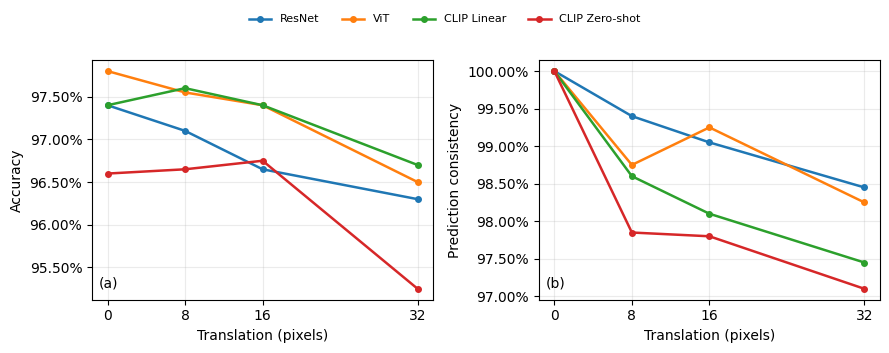
\includegraphics[width=\linewidth]
    {translation_curves.png}
    \caption{Translation accuracy and prediction consistency across 0--32 px displacements.}
    \label{fig:translation}
\end{figure}

ResNet, ViT, and CLIP are all mostly robust to translation, as can be seen by the accuracy for each decreasing only slightly from the clean baseline even at the maximum 32px translation. Consistency on the other hand did decline more than accuracy, but that too only by a slight margin. ResNet retained the highest consistency and CLIP Linear the highest accuracy relative to baseline at 32px. However, the patch shuffle experiment led to a greater decrease in accuracy across all the representations as seen in Table~\ref{tab:task1_interventions}, with ViT being the most robust compared to the rest and CLIP Zero-shot the least. The differences in model performance due to translation versus patch shuffle could potentially be explained by the difference in maintaining global structure across each transformation. In translation, the object's position is just shifted slightly but the overall structure of the image remains preserved globally unlike in patch shuffling, where locality may be preserved due to patches but the shuffling destroys global structure. This in turn implies that these models, especially CLIP,  seemingly depend more on spatial organization for predictions compared to positional information.


\subsubsection{Representation Analysis}
\label{subsubsec:results-t1-representation}

% Report cosine stability.
% Include t-SNE or UMAP visualization.
\begin{figure*}[t]
    \centering
    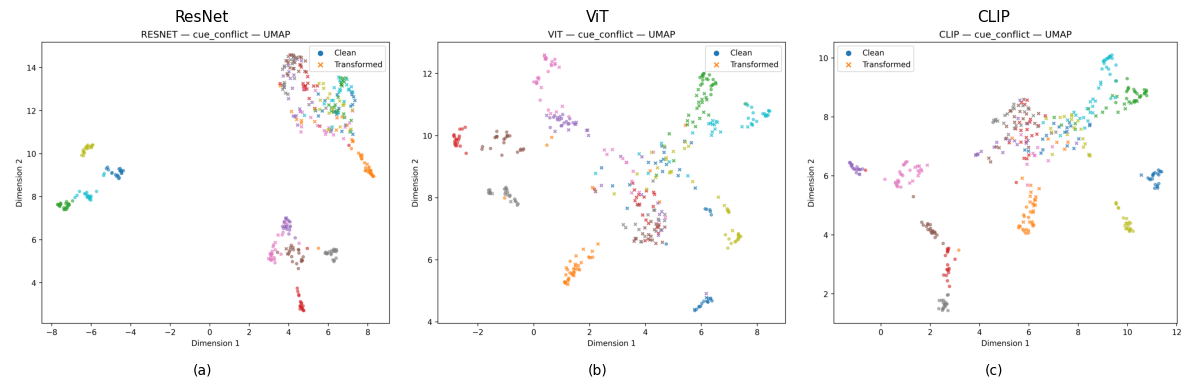
\includegraphics[width=0.88\textwidth]
    {umap_cue.png}
    \caption{UMAP of clean and cue-conflict representations for ResNet, ViT, and CLIP; colors denote ground-truth classes and markers distinguish clean from cue-conflict representations.}
    \label{fig:cue_umap}
\end{figure*}
% Discuss prediction/representation agreements or mismatches.
\begin{figure*}[t]
    \centering
    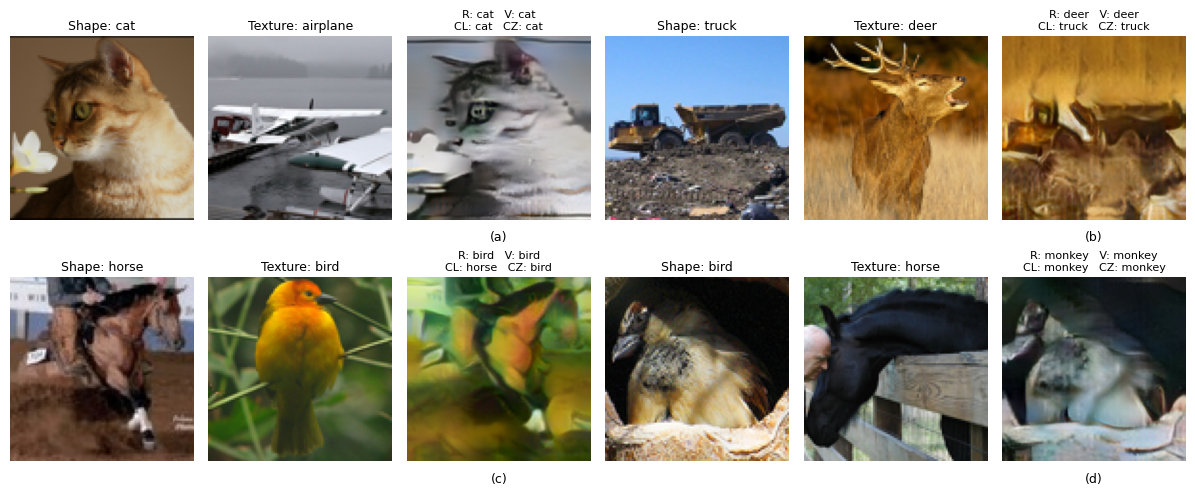
\includegraphics[width=\textwidth]
    {cue_conflicts2.png}
    \caption{Selected cue-conflict examples and model predictions. R = ResNet, V = ViT, CL = CLIP Linear, and CZ = CLIP Zero-shot.}
    \label{fig:cue_examples}
\end{figure*}

\begin{table}[t]
\centering
\caption{Mean cosine similarity between clean and transformed representations; higher values indicate greater stability.}
\label{tab:repr_stability}
\scriptsize
\setlength{\tabcolsep}{3pt}
\begin{tabular}{lcccccc}
\toprule
Backbone & Gray & T8 & T16 & T32 & Patch & Cue \\
\midrule
ResNet & .800 & .967 & .951 & .930 & .695 & .236 \\
ViT    & .731 & .944 & .975 & .943 & .628 & .232 \\
CLIP   & .880 & .978 & .964 & .966 & .756 & .705 \\
\bottomrule
\end{tabular}
\end{table}

The UMAP representations as well as similarity scores in Table~\ref{tab:repr_stability} help us further understand to what extent the discussed prediction level changes agree with the feature representation changes. In the case of Translation, the representation similarity scores are high as well as the prediction consistency across all models which implies a good degree of agreement between the two. On the other hand, a good example of a case of mismatch would be CLIP's representation similarity being the highest for patch shuffle while the accuracy results for both CLIP Linear and Zero-shot were the lowest. This could be explained by how even a smaller change in feature representation could potentially change features which the model considered important for classification, hence directly affecting its prediction abilities. CLIP Linear and CLIP Zero-Shot also further help us understand the impact of using the same core feature representation but varying the classifier, with our results across all aforementioned interventions being similar for both likely due to the shared encoder, but the impact of difference in classifiers still shows in cases such as cue-conflicts. (Figure 3c, Linear favours shape, Zero-shot texture)  

From the obtained results, we can infer that for differences in results between ResNet versus ViT, architecture is likely a contributor. Whereas for ViT vs CLIP, architecture alone cannot explain differences and they may be attributed to the pretraining data or supervision.


\subsection{Task 2: Unsupervised Domain Adaptation}
\label{subsec:results-task2}



\begin{table*}[t]
\centering
\caption{Task 2 source and Sketch performance and domain separability. A/F1 denotes accuracy/macro-F1; values are percentages.}
\label{tab:task2_main}
\scriptsize
\setlength{\tabcolsep}{3.2pt}
\begin{tabular}{lccccccc}
\toprule
Method &
Photo A/F1 &
Art A/F1 &
Cartoon A/F1 &
Mean Src. A/F1 &
Sketch A/F1 &
$\Delta$ Sketch &
Sep. \\
\midrule
Source-only &
96.7/96.1 &
92.7/92.4 &
95.5/96.0 &
95.0/94.8 &
66.2/68.2 &
0.0 &
100.0 \\

DAN &
97.0/96.4 &
92.7/93.0 &
94.5/94.9 &
94.7/94.7 &
70.7/65.6 &
+4.6 &
83.2 \\

DANN &
96.7/96.1 &
89.8/89.6 &
94.2/94.3 &
93.6/93.3 &
39.6/37.7 &
-26.6 &
99.6 \\

CDAN &
95.2/94.3 &
89.5/89.3 &
93.2/93.5 &
92.6/92.4 &
44.5/45.9 &
-21.6 &
99.2 \\
\bottomrule
\end{tabular}
\end{table*}

For the Source-only ERM, the source-to-target domain gap is large with sketch accuracy dropping by 28.8 percentage points compared to mean source accuracy. The weakest sketch classes can be identified as giraffe (46.7\%), horse (48.8\%), person (59.4\%), and house (60.0\%), with the model predicting images with a horse and a giraffe as "dog" in 286 and 184 cases respectively. Hence, we can deduce that the (source-only) model is unable to generalize well to the new sketch domain based on the drop in performance.


\subsubsection{Domain Alignment and Class-Level Effects}
\label{subsubsec:results-t2-alignment}
Relative to this source-only target accuracy, only DAN was able to produce an increase in target accuracy by 4.56 \% points with source accuracy similar to source-only at 94.72\%. The domain separability fell to 0.832 as well, so in this case we could possibly attribute the increased target accuracy to decreased domain separability and perhaps even successful adaptation, but it cannot be claimed that said decrease was the sole cause of improved target performance. Moreover, the slight decrease in macro-F1 for DAN despite increased accuracy reveals that the model may be performing well on only a few select classes but not every class in the domain for example house(+40.0 \% points) compared to dog (-21.0\% points).

On the other hand, DANN and CDAN produce significantly lower sketch accuracy compared to source-only, despite only a very slight decrease in source accuracy and in both cases the domain separability barely decreased and was higher than DAN. Upon looking into the class-level results, we found that for DANN elephant fell from 90\% to 0\% while person improved by about 35 points, and for CDAN, dog fell by about 50.6 points while house rose to 100\%. These results suggest negative transfer, which in turn may be due to unstable training, which was tracked using a feature variance score. For DANN, variance rose from 1.87 to 59.49 despite normalisation, and domain loss was maintained at 0.70 which implies the discriminator was performing poorly. For CDAN, the variance rose from 9.73 to a high 3583.05 in one epoch, reflecting unstable training. It must be noted that for CDAN raw features were used, unlike DANN so a direct comparison of the two is not possible. 

Moreover, due to training instability in DANN and CDAN, comparing class-conditional alignment to marginal alignment proves to be difficult. From the obtained results (Figure~\ref{fig:task2_evidence}), we can observe that DAN had improved target performance but CDAN was unable to preserve class structure, with dog falling by about 50.6 points and elephant by about 33.8. On the other hand, CDAN's overall sketch accuracy was better than DANN and its worst drop at class-level for "dog" was smaller in comparison to DANN for "elephant". However, we cannot make any claims about conditioning compared to marginal due to the main limitation of normalised versus raw features in DANN and CDAN respectively, the aforementioned instability, and also the difference in type of loss used for DAN versus CDAN (MMD loss vs adversarial).

% \begin{figure*}[t]
%     \centering
%     \includegraphics[width=0.80\textwidth]
%     {task2_evidence.png}
%     \caption{[Your caption describing (a) per-class Sketch accuracy changes and (b) the DAN alignment-strength study.]}
%     \label{fig:task2_diagnostics}
% \end{figure*}

% \begin{figure*}[t]
%     \centering
%     \includegraphics[width=0.72\textwidth]
%     {task2_latest.png}
%     \caption{[Your caption describing classification and adaptation losses for Source-only, DAN, DANN, and CDAN. Note the log-scaled loss axis.]}
%     \label{fig:task2_training}
% \end{figure*}

% \begin{figure*}[t]
%     \centering

%     \includegraphics[width=0.49\textwidth]
%     {task2_evidence.png}
%     \hfill
%     \includegraphics[width=0.49\textwidth]
%     {task2_latest.png}

%     \caption{[Your caption describing the left diagnostic figure and the right training-loss figure.]}
%     \label{fig:task2_evidence}
% \end{figure*}

\begin{figure*}[t]
    \centering

    % ---------------- LEFT SIDE ----------------
    \begin{minipage}[b]{0.48\textwidth}
        \centering

        % Compact lambda table
        \scriptsize
        \setlength{\tabcolsep}{3pt}
        \begin{tabular}{ccccc}
        \toprule
        $\lambda_{\mathrm{MMD}}$ &
        Src. A/F1 &
        Sketch A/F1 &
        $\Delta$ Sketch &
        Sep. \\
        \midrule
        0.1 & 96.3/96.3 & 71.6/67.7 & +5.5 & 74.0 \\
        1   & 94.7/94.7 & 70.7/65.6 & +4.6 & 83.2 \\
        10  & 21.7/5.1  & 4.1/1.1   & -62.1 & 59.1 \\
        \bottomrule
        \end{tabular}

        \vspace{0.3em}

        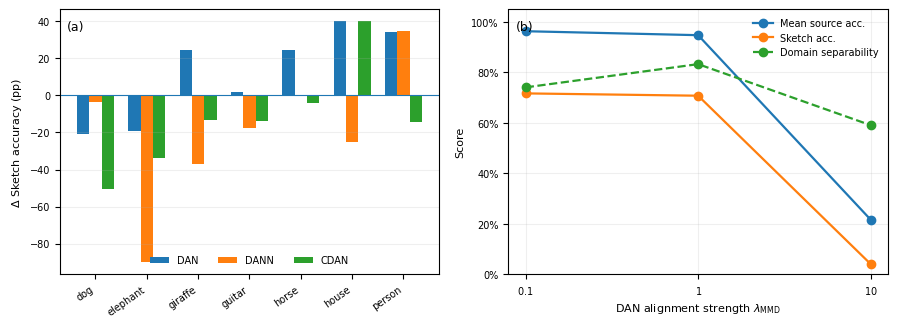
\includegraphics[width=\linewidth]
        {task2_evidence.png}
    \end{minipage}
    \hfill
    % ---------------- RIGHT SIDE ----------------
    \begin{minipage}[b]{0.49\textwidth}
        \centering
        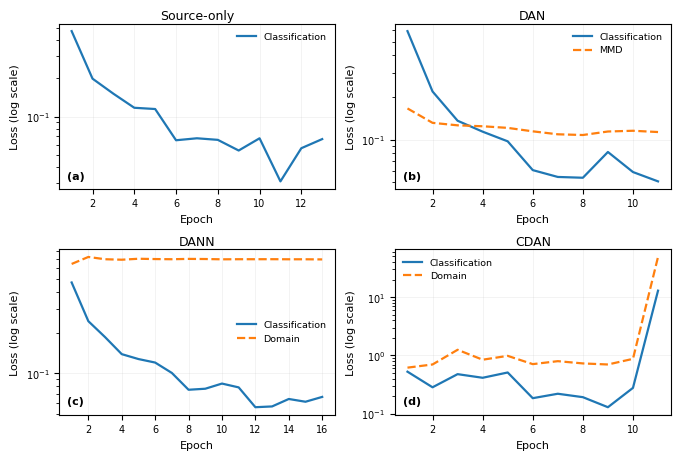
\includegraphics[width=\linewidth]
        {task2_latest.png}
    \end{minipage}

    \caption{Task 2 diagnostics: controlled DAN alignment-strength study and per-class Sketch changes (left), with training losses for Source-only, DAN, DANN, and CDAN (right).}
    \label{fig:task2_evidence}

\end{figure*}


\subsubsection{Controlled Alignment-Strength Study}
\label{subsubsec:results-t2-controlled}


The results in Figure~\ref{fig:task2_evidence} show that increasing alignment strength from 0.1 to 1 surprisingly led to a decrease in both source and sketch accuracy, while domain separability increased. Increasing strength further to 10 gave extreme results, with source and target accuracy dropping greatly to 21.7 and 4.1, while the separability also decreased. The results at $\lambda =10 $ suggest over-alignment, and the overall pattern suggests how increasing alignment strength degrades both source and target performance, perhaps due to domains being aligned in a manner which results in important information such as class-discriminative features being lost. Based on these results, $\lambda=0.1$ could have been selected without consulting target labels because it has the highest mean source-validation macro-F1 of the three at 96.34\%.


\subsection{Task 3: Domain Generalization}
\label{subsec:results-task3}

\begin{table*}[t]
\centering
\caption{Task 3 source and Sketch performance, source-domain separability, and sharpness. A/F1 denotes accuracy/macro-F1; Sep. denotes separability and Sharp. the sharpness proxy.}
\label{tab:task3_main}
\scriptsize
\setlength{\tabcolsep}{2.6pt}
\renewcommand{\arraystretch}{0.92}

\begin{tabular}{lccccccccc}
\toprule
Method &
Photo A/F1 &
Art A/F1 &
Cartoon A/F1 &
Mean Src. A/F1 &
Worst Src. A/F1 &
Sketch A/F1 &
$\Delta$ Sk. &
Sep. &
Sharp. \\
\midrule

ERM &
96.7/96.1 &
92.7/92.4 &
95.5/96.0 &
95.0/94.8 &
92.7/92.4 &
66.2/68.2 &
0.0 &
92.0 &
.279 \\

DAN-DG &
25.7/5.9 &
22.0/5.1 &
17.3/4.2 &
21.7/5.1 &
17.3/4.2 &
4.1/1.1 &
-62.1 &
33.2 &
.012 \\

SAM &
97.6/97.2 &
92.7/92.6 &
95.5/96.0 &
95.3/95.2 &
92.7/92.6 &
53.0/56.0 &
-13.2 &
91.0 &
.141 \\

\bottomrule
\end{tabular}
\end{table*}



\begin{figure*}[t]
    \centering

    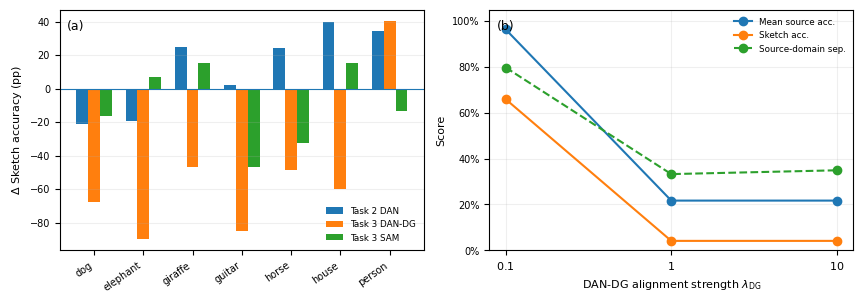
\includegraphics[width=0.455\textwidth]
    {task3_graphs.png}
    \hfill
    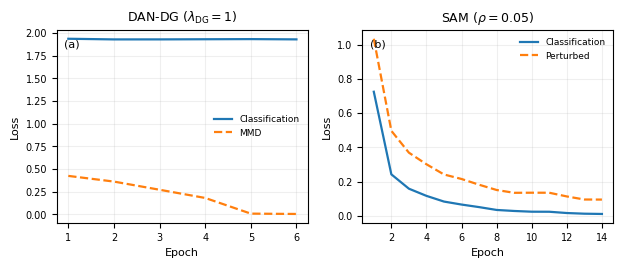
\includegraphics[width=0.535\textwidth]
    {task3_plots.png}

    \caption{Task 3 diagnostics: training curves (left), and per-class Sketch changes with the DAN-DG alignment-strength study (right).}
    \label{fig:task3_evidence}
\end{figure*}
\subsubsection{Generalization Performance}
\label{subsubsec:results-t3-performance}

Table~\ref{tab:task3_main} shows ERM had best sketch accuracy relative to mean source accuracy, followed by SAM. However, it must be noted how SAM had lower sketch accuracy (by 13.2 \% points) despite having slightly higher mean source accuracy and nearly identical worst-source accuracy compared to ERM. Hence, we cannot predict performance on unseen domain based solely on source performance, but it can provide an idea of said performance such as in the case of DAN-DG. DAN-DG has very poor mean source accuracy relative to ERM and SAM, and this is also followed by poor sketch accuracy. These aggregate results provide useful information but class-level results need to be inspected in order to get a more complete picture, such as the notable difference in sketch accuracies for each class as seen in Figure~\ref{fig:task3_evidence}. For example, in SAM's case, "guitar" sketch accuracy drops by 46.5 \% points relative to ERM with guitars being predicted as elephants in 202 cases, while "giraffe" accuracy increases by 15.5 \% points. This is not visible from SAM's source performance metrics alone, which were similar to ERM.



\subsubsection{Domain Separability and Sharpness}
\label{subsubsec:results-t3-diagnostics}


Apart from source-accuracy metrics domain separability scores were also computed, as can be seen in Table~\ref{tab:task3_main}. DAN-DG achieved a low separability score of 33.2\%, which implies that the source domains were made nearly completely indistinguishable by DAN-DG, but the resulting sketch accuracy drop of 62.1 percentage points relative to ERM shows that domain invariance did not improve Sketch recognition. This is supported by the graph in Figure~\ref{fig:task3_evidence}, which shows the classification loss as nearly constant at 1.93 (chance-level) throughout training while the MMD loss is reduced from 0.42 to nearly 0. Furthermore, class-level results show that the model predicts every Sketch image as ``person'', irrespective of which class it actually belongs to, indicating that the model has lost the ability to distinguish between classes. This could be caused by the increased alignment strength, which can be further supported by our controlled experiment on $\lambda$ in which increasing lambda from 0.1 to 1 resulted in source and sketch accuracy collapsing, suggesting how stronger alignment may have removed class-discriminative information.

Moving on to the sharpness results, we find that SAM was able to reduce the common sharpness proxy from 0.2795 to 0.1411 relative to ERM, but unexpectedly sketch performance decreased from 66.2 to 52.97\%. This implies that in this experiment decreasing the sharpness did not help improve sketch performance, which may be explained by how the sharpness proxy only measures how stable the source loss is when model parameters are slightly perturbed, not how robust it is to a changed input domain entirely. Apart from that, DAN-DG has a lower sharpness proxy compared to SAM, but this is more so because DAN-DG's loss was already very high due to the aforementioned model collapse. This helps us realize the importance of interpreting sharpness proxy results alongside classification loss values, because exceptions such as model collapse may result in misleading results.


% ------------------------------------------------------------
% TASK 4 RESULTS
% ------------------------------------------------------------

\subsection{Task 4: Open-Set Recognition}
\label{subsec:results-task4}

\subsubsection{Post-hoc Novelty Detection}
\label{subsubsec:results-t4-posthoc}


Four types of post-hoc novelty scores were used to obtain a measure of unknownness: MSP measuring normalized confidence, MLS the absolute maximum logit, Energy the evidence from all logits, and Mahalanobis the feature-space distance. Our results show how MSP gives the best near AUROC at 81.64\% but the lowest far-rejection rate at 44.5\%, which could imply that normalized confidence seems to provide the most useful information for distinguishing between known and near-unknown examples but it cannot provide as strong a measure for rejecting far-unknowns. Logit-based scores unsurprisingly appear to be most informative about rejecting both near and far unknowns based on the similar highest near rejection and far rejection rates for MLS and Energy. Lastly, as evidenced by Mahalanobis giving the highest Far and All AUROC scores, feature-space distance seems to be useful in ranking far unknowns specifically, which is in line with how very semantically different unknowns would be expected to lie far from known feature clusters. Overall these scores mostly agree across thresholds, but there is a notable disagreement between Mahalanobis and Energy, with Mahalanobis having a higher far AUROC score but lower far rejection compared to Energy, which suggests how single threshold performance may differ compared to ranking across thresholds.


% ============================================================
% TASK 4: BOTH REQUIRED TABLES IN ONE COMPACT FLOAT
% ============================================================

\begin{table*}[t]
\centering
\caption{Task 4 OSR results. N/F denotes near/far, K-Acc. known acceptance, Rej. rejection rate, and PH the placeholder score; values are percentages.}
\label{tab:task4_results}
\scriptsize
\setlength{\tabcolsep}{2.3pt}
\renewcommand{\arraystretch}{0.90}

\begin{minipage}[t]{0.485\textwidth}
\centering
\textbf{(a) Frozen Vanilla score comparison}

\vspace{0.2em}
\begin{tabular}{lrrrrrr}
\toprule
Score &
N-AUC &
F-AUC &
All &
K-Acc. &
N-Rej. &
F-Rej. \\
\midrule
MSP & 81.64 & 89.33 & 85.48 & 94.78 & 31.50 & 44.50 \\
MLS & 79.84 & 88.19 & 84.01 & 94.98 & 32.50 & 52.50 \\
Energy & 79.83 & 88.21 & 84.02 & 95.06 & 32.13 & 53.00 \\
Mah. & 80.23 & 91.76 & 86.00 & 94.76 & 29.50 & 52.13 \\
\bottomrule
\end{tabular}
\end{minipage}
\hfill
\begin{minipage}[t]{0.505\textwidth}
\centering
\textbf{(b) Trained-model comparison}

\vspace{0.2em}
\begin{tabular}{lrrrrrr}
\toprule
Model/Score &
CSA &
N-AUC &
F-AUC &
K-Acc. &
N-Rej. &
F-Rej. \\
\midrule
Vanilla/MLS & 94.79 & 79.84 & 88.19 & 94.98 & 32.50 & 52.50 \\
GCSC/MLS & 95.18 & 81.43 & 90.14 & 94.48 & 36.13 & 60.00 \\
PROSER/MLS & 94.22 & 79.86 & 84.87 & 95.18 & 35.13 & 42.13 \\
PROSER/PH & 94.22 & 79.08 & 87.90 & 94.95 & 34.00 & 49.13 \\
\bottomrule
\end{tabular}
\end{minipage}

\end{table*}


% ============================================================
% TASK 4: REQUIRED SCORE-DISTRIBUTION FIGURE
% ============================================================

\begin{figure*}[t]
    \centering
    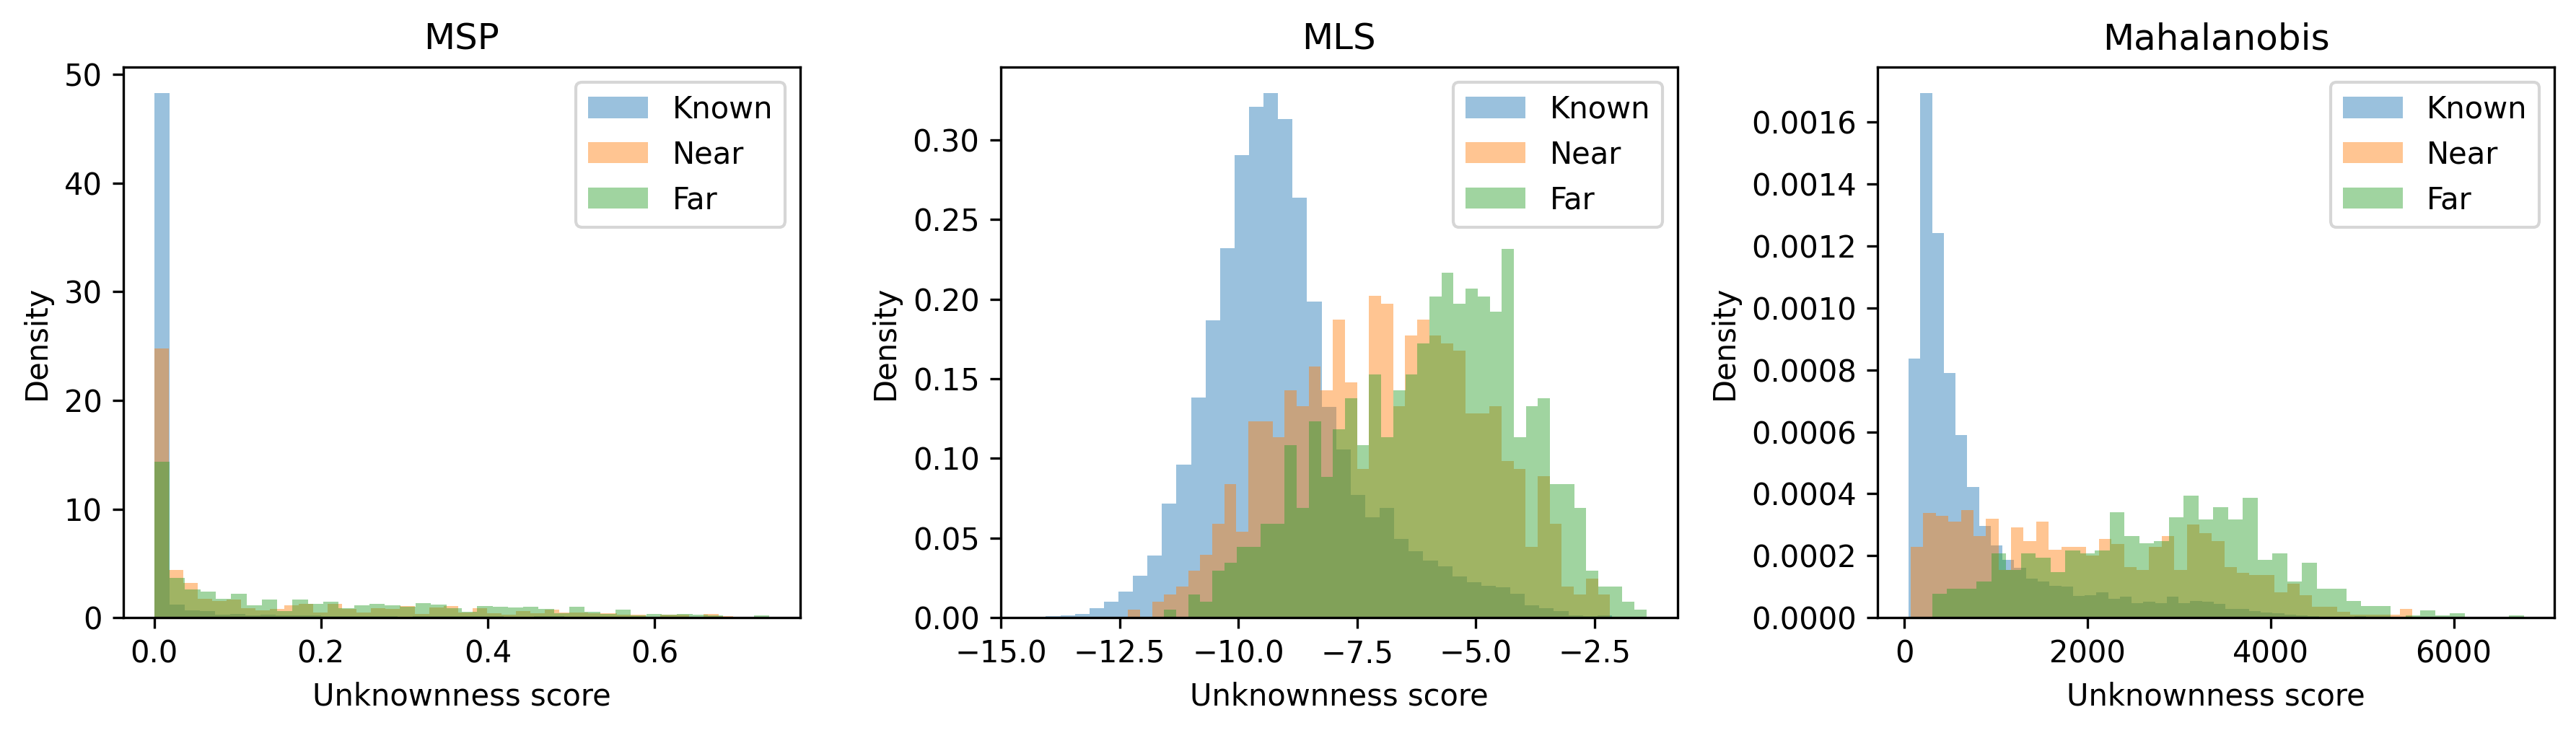
\includegraphics[width=0.80\textwidth]{task4_evidence.png}
    \caption{Unknownness-score distributions for known, near-unknown, and far-unknown inputs using MSP, MLS, and Mahalanobis.}
    \label{fig:task4_scores}
\end{figure*}


\subsubsection{Vanilla, GCSC, and PROSER}
\label{subsubsec:results-t4-models}

% Compare:
% - closed-set accuracy
% - near-unknown rejection
% - far-unknown rejection
% - MLS performance
% - PROSER placeholder score
Next, we evaluated GCSC on closed-set accuracy and open-set recognition performance, with Table~\ref{tab:task4_results} showing how GCSC MLS had increased CSA, AUROC scores, and near and far rejection rates compared to Vanilla MLS. Hence the random augmentations used by GCSC helped improve both CSA and open-set recognition, which can possibly be explained by how augmentation helps produce more robust known-class regions. However, its effect remains similar to Vanilla for near and far unknowns with near unknowns remaining harder to reject, as evidenced by  the larger increase in far rejection (7.5 \% points) compared to near (3.6 \% points).

On the other hand, PROSER is able to improve near rejection slightly by 2.6\% points compared to Vanilla, but cannot perform as well on near rejection as GCSC. Far rejection is also worse than both Vanilla and GCSC, and PROSER also has lower CSA by 0.57 and 0.96 \% points relative to Vanilla and GCSC respectively. However, comparing PROSER's own Placeholder versus MLS scores reveals an increase of 7.0 \% points in far rejection for placeholder compared to MLS, which indicates that learned placeholder responses provide useful information for detection, particularly for far unknowns. However, we cannot claim that they successfully tightened the boundaries between known classes because the overall performance compared to Vanilla and GCSC did not show improvement across most metrics. Moreover, importantly interpolation between known classes did not consistently result in improvement in unknown rejection especially for far unknowns, which may indicate that the mixed-class constructed unknowns did not represent the actual unknowns as well as could be expected.

\subsubsection{Near- and Far-Unknown Failure Analysis}
\label{subsubsec:results-t4-failures}

From Table~\ref{tab:task4_results} we can see how with vanilla MLS the rate of near rejection is 32.5\% compared to a higher rate of far rejection at 52.5\%. This is in line with the idea of semantic similarity making unknowns harder to reject for the model, and this is further supported by our class-level analysis. The most often accepted near classes include "pickup truck" (at 88\% acceptance rate) which is absorbed by the CIFAR-10 label "automobile", "bus" (85\%) as "truck", and "wolf" (76\%) as "dog". The labels predicted by the model for these near-unknowns may not be correct but they do make sense semantically, especially in the case of pickup truck and automobile, and bus and truck. However, the most commonly accepted far unknowns include "wardrobe" (65\%) as "truck", "mushroom" (63\%) as "bird", and "clock" (46\%) as "automobile". These predicted labels , on the other hand, are difficult to explain as there appears to be very little semantically similar about birds and mushrooms for example. It can therefore be deduced that generally near unknowns are harder to reject possibly due to semantic overlap, but the lack of said overlap does not seem to be sufficient to reject far unknowns.

\begin{table}[t]
    \centering
    \scriptsize
    \setlength{\tabcolsep}{3pt}
    \textbf{Selected Vanilla MLS unknown failures.}\\[0.2em]
    \begin{tabular}{llrr}
        \toprule
        Group & Unknown $\rightarrow$ predicted known & Score & Threshold \\
        \midrule
        Near & bus $\rightarrow$ truck & -12.325 & -5.871 \\
        Near & fox $\rightarrow$ cat & -11.784 & -5.871 \\
        Near & wolf $\rightarrow$ dog & -11.414 & -5.871 \\
        Far & wardrobe $\rightarrow$ truck & -11.564 & -5.871 \\
        Far & bottle $\rightarrow$ cat & -10.748 & -5.871 \\
        Far & mushroom $\rightarrow$ bird & -10.460 & -5.871 \\
        \bottomrule
    \end{tabular}
\end{table}


% ============================================================
% CROSS-TASK DISCUSSION
% ============================================================

\section{Cross-Task Discussion}
\label{sec:discussion}


\textbf{Visual cues and distribution shift:}
Task 1 results helped us understand how colour and spatial interventions generally resulted in a decrease in performance accuracy for each model, albeit of differing magnitudes depending on type of intervention and model, and cue-conflicts showed how models differed in how strongly they relied on texture versus shape. Hence, we can connect this to the failure patterns observed under PACS domain shifts because the shift from source domains Photo/Art/Cartoon to Sketch also involves changes in colour as well as texture. The sketch performance drop in both tasks 2 and 3 is therefore consistent with the decrease in accuracy in Task 1, but we can only interpret this qualitatively as datasets and architectures differ across tasks.

\textbf{Invariance versus discriminability:}
As extensively explored in Sections~\ref{subsubsec:results-t2-alignment} and~\ref{subsubsec:results-t3-diagnostics}, the experiments conducted in tasks 2 and 3 established that reduced domain separability was not sufficient for improved classification in our study. In Task 2, DAN reducing separability was accompanied by improved sketch performance, hence a certain level of domain invariance is useful but due to limitations we cannot claim causality on its own. Task 3 further showed how excessive alignment can result in lower domain separability scores but also a loss of class-discriminative information, hence a careful balance must be maintained to achieve the true goal of domain invariance.

\textbf{Importance of target domain access:} The results show Task2 DAN with a $\Delta$ vs ERM = +0.0456, showing slight but present improvement over the ERM baseline sketch accuracy, whereas for Task3 DAN-DG we have $\Delta$ vs ERM = -0.6210, a significant drop in sketch accuracy. However, this comparison alone is not sufficient to claim that solely access to Sketch allows more useful alignment, because alignment strength($\lambda$) appears to have a huge effect on the model’s classification ability in the case of DAN-DG. Said effect can be clearly observed by the difference in sketch accuracy when lambda was set to 0.1, producing a value of 0.6589 which is nearly the same as ERM’s sketch accuracy. Hence, due to limitations such as the alignment strength factor, as well as differences in source domain alignment in each task we cannot attribute definite causality to target access. However, the large difference between DAN and DAN-DG does provide evidence for target access being useful, it just does not establish causality.

\textbf{Task 4 Synthesis: }
Section~\ref{subsec:results-task4} already discusses Vanilla, GCSC and PROSER and their CSA versus unknown rejection performances in detail, but upon concluding the four main experiments in this study a certain pattern can be seen emerging as we collect the results for each task. Strong performance on the metrics chosen at training time does not necessarily mean that the representations producing this performance also perform well during inference. A few examples are the much lower sketch accuracy for DANN and CDAN compared to the stable source accuracy similar to ERM in task 2 - though as discussed in Section~\ref{subsubsec:results-t2-alignment}, this may reflect training instability - the lower sharpness score achieved by SAM in task 3 not accompanied by an improved sketch accuracy, and finally the better CSA and AUROC in GCSC in task 4, which produced smaller improvement in near unknown rejection compared to far.



\textbf{Overall Synthesis:}
Looking at our findings across all four tasks reveals several important patterns and useful information regarding what needs to be preserved, what should become invariant, and lastly what should be discarded when it comes to a robust representation. Firstly, we understand that a representation must preserve information or features which primarily help distinguish between classes, with a strong example being shape and overall structure of image. Colour, texture, and other visual cues may also be important, but Task 1 results showed the greatest drop in accuracy upon patch shuffling for ResNet and CLIP, showing the significance of global structure specifically. The importance of preserving such class-discriminative information is then in turn shown by the results for the alignment strength DAN-DG experiment in Task 3, which shows how excessive alignment may lead to loss of class-discriminative information and in turn result in model collapse. Secondly, the representation should also become invariant to small changes in appearance of input, such as colour changes which do not modify the main class-identifying features, or small positional changes like the 8px translation we conducted in Task 1. A similar principle was used to test domain invariance in Task 2 by using moderate alignment of source domains with the target sketch domain, with the resulting improved target performance possibly being explained by increased domain invariance.
Lastly, Task 4 primarily helps us identify the inputs which should be rejected by a model, namely those images which do not belong to a class known by the model. However, the limitations when performing such rejections are that rejection is not always based on just the quality of the representation, but on the position of the unknown in the label space. This is one of our primary findings from task 4, where near-unknowns were markedly harder to reject than far-unknowns.


\section{Conclusion}
\label{sec:conclusion}
All in all, the four broad experiments conducted in this study covered inductive biases and visual cues, domain shifts and importance of domain invariance, and lastly rejection of semantic novelty. Our findings revealed how robust representations should preserve class-discriminative information, tolerate minor non-interfering changes in input appearance, while being careful to not let excessive alignment strategies destroy mentioned discriminative information. Moreover, CSA-rejection tradeoff was studied and it was discovered how higher closed-set accuracy did not necessarily translate to better unknown rejection, especially for semantically near unknowns.


\bibliographystyle{plainnat}
\bibliography{citations}

\appendix
\section{Formulae}
\label{app:formulae}

\begin{equation}
\text{Shape Bias}(\%) = \frac{N_{\text{shape}}}{N_{\text{shape}} + N_{\text{texture}}} \times 100
\label{eq:shape_bias}
\end{equation}

\begin{equation}
\text{Coverage}(\%) = \frac{N_{\text{shape}} + N_{\text{texture}}}{N_{\text{total}}} \times 100
\label{eq:coverage}
\end{equation}

\begin{equation}
\text{Consistency}(\delta) = \frac{1}{N} \sum_{i=1}^{N} \mathbb{1}\left[\hat{y}(x_i) = \hat{y}(T_\delta(x_i))\right]
\label{eq:consistency}
\end{equation}

\begin{equation}
I_T = \frac{1}{N} \sum_{i=1}^{N} \frac{f(x_i)^\top f(T(x_i))}{\lVert f(x_i) \rVert_2 \, \lVert f(T(x_i)) \rVert_2}
\label{eq:cosine_stability}
\end{equation}

\begin{equation}
\mathcal{L}_{\text{DAN}} = \mathcal{L}_{\text{cls}} + \lambda_{\text{MMD}} \left\lVert \mathbb{E}_s[\phi(F(x_s))] - \mathbb{E}_t[\phi(F(x_t))] \right\rVert^2_{\mathcal{H}}
\label{eq:mmd}
\end{equation}

\begin{equation}
\alpha(p) = \frac{2}{1 + \exp(-10p)} - 1
\label{eq:grl}
\end{equation}

\begin{equation}
g(x) = \text{vec}(f \otimes p), \quad f = F(x),\ p = C(f)
\label{eq:cdan}
\end{equation}

\begin{equation}
\mathcal{L}_{\text{DAN-DG}} = \mathcal{L}_{\text{ERM}} + \frac{\lambda_{\text{DG}}}{3} \sum_{e < e'} \text{MMD}^2\left(F(X_e), F(X_{e'})\right)
\label{eq:dandg}
\end{equation}

\begin{equation}
U_{\mathrm{MSP}}(x)
=
1 - \max_{k}
\frac{\exp(z_k(x))}
{\sum_{j=1}^{K}\exp(z_j(x))}
\label{eq:msp}
\end{equation}

\begin{equation}
U_{\mathrm{MLS}}(x)
=
-\max_{k} z_k(x)
\label{eq:mls}
\end{equation}

\begin{equation}
U_{\mathrm{Energy}}(x)
=
-T \log
\sum_{k=1}^{K}
\exp\left(\frac{z_k(x)}{T}\right),
\qquad T=1
\label{eq:energy}
\end{equation}

\begin{equation}
U_{\mathrm{Mah}}(x)
=
\min_{k}
\left(f(x)-\mu_k\right)^\top
\Sigma^{-1}
\left(f(x)-\mu_k\right)
\label{eq:mahalanobis}
\end{equation}

\begin{equation}
\mu_k
=
\frac{1}{N_k}
\sum_{i:y_i=k} f(x_i)
\label{eq:mahalanobis_mean}
\end{equation}


\end{document}